\documentclass[handout,noauthor]{../ximera}

\graphicspath{  
{./}
{./whoAreYou/}
{./drawingWithTheTurtle/}
{./bisectionMethod/}
{./circles/}
{./anglesAndRightTriangles/}
{./lawOfSines/}
{./lawOfCosines/}
{./plotter/}
{./staircases/}
{./pitch/}
{./qualityControl/}
{./symmetry/}
{./nGonBlock/}
}


%% page layout
\usepackage[cm,headings]{fullpage}
\raggedright
\setlength\headheight{13.6pt}


%% fonts
\usepackage{euler}

\usepackage{FiraMono}
\renewcommand\familydefault{\ttdefault} 
\usepackage[defaultmathsizes]{mathastext}
\usepackage[htt]{hyphenat}

\usepackage[T1]{fontenc}
\usepackage[scaled=1]{FiraSans}

%\usepackage{wedn}
\usepackage{pbsi} %% Answer font


\usepackage{cancel} %% strike through in pitch/pitch.tex


%% \usepackage{ulem} %% 
%% \renewcommand{\ULthickness}{2pt}% changes underline thickness

\tikzset{>=stealth}

\usepackage{adjustbox}

\setcounter{titlenumber}{-1}

%% journal style
\makeatletter
\newcommand\journalstyle{%
  \def\activitystyle{activity-chapter}
  \def\maketitle{%
    \addtocounter{titlenumber}{1}%
                {\flushleft\small\sffamily\bfseries\@pretitle\par\vspace{-1.5em}}%
                {\flushleft\LARGE\sffamily\bfseries\thetitlenumber\hspace{1em}\@title \par }%
                {\vskip .6em\noindent\textit\theabstract\setcounter{question}{0}\setcounter{sectiontitlenumber}{0}}%
                    \par\vspace{2em}
                    \phantomsection\addcontentsline{toc}{section}{\thetitlenumber\hspace{1em}\textbf{\@title}}%
                     }}
\makeatother



%% thm like environments
\let\question\relax
\let\endquestion\relax

\newtheoremstyle{QuestionStyle}{\topsep}{\topsep}%%% space between body and thm
		{}                      %%% Thm body font
		{}                              %%% Indent amount (empty = no indent)
		{\bfseries}            %%% Thm head font
		{)}                              %%% Punctuation after thm head
		{ }                           %%% Space after thm head
		{\thmnumber{#2}\thmnote{ \bfseries(#3)}}%%% Thm head spec
\theoremstyle{QuestionStyle}
\newtheorem{question}{}



\let\freeResponse\relax
\let\endfreeResponse\relax

%% \newtheoremstyle{ResponseStyle}{\topsep}{\topsep}%%% space between body and thm
%% 		{\wedn\bfseries}                      %%% Thm body font
%% 		{}                              %%% Indent amount (empty = no indent)
%% 		{\wedn\bfseries}            %%% Thm head font
%% 		{}                              %%% Punctuation after thm head
%% 		{3ex}                           %%% Space after thm head
%% 		{\underline{\underline{\thmname{#1}}}}%%% Thm head spec
%% \theoremstyle{ResponseStyle}

\usepackage[tikz]{mdframed}
\mdfdefinestyle{ResponseStyle}{leftmargin=1cm,linecolor=black,roundcorner=5pt,
, font=\bsifamily,}%font=\wedn\bfseries\upshape,}


\ifhandout
\NewEnviron{freeResponse}{}
\else
%\newtheorem{freeResponse}{Response:}
\newenvironment{freeResponse}{\begin{mdframed}[style=ResponseStyle]}{\end{mdframed}}
\fi



%% attempting to automate outcomes.

%% \newwrite\outcomefile
%%   \immediate\openout\outcomefile=\jobname.oc
%% \renewcommand{\outcome}[1]{\edef\theoutcomes{\theoutcomes #1~}%
%% \immediate\write\outcomefile{\unexpanded{\outcome}{#1}}}

%% \newcommand{\outcomelist}{\begin{itemize}\theoutcomes\end{itemize}}

%% \NewEnviron{listOutcomes}{\small\sffamily
%% After answering the following questions, students should be able to:
%% \begin{itemize}
%% \BODY
%% \end{itemize}
%% }
\usepackage[tikz]{mdframed}
\mdfdefinestyle{OutcomeStyle}{leftmargin=2cm,rightmargin=2cm,linecolor=black,roundcorner=5pt,
, font=\small\sffamily,}%font=\wedn\bfseries\upshape,}
\newenvironment{listOutcomes}{\begin{mdframed}[style=OutcomeStyle]After answering the following questions, students should be able to:\begin{itemize}}{\end{itemize}\end{mdframed}}



%% my commands

\newcommand{\snap}{{\bfseries\itshape\textsf{Snap!}}}
\newcommand{\flavor}{\link[\snap]{https://snap.berkeley.edu/}}
\newcommand{\mooculus}{\textsf{\textbf{MOOC}\textnormal{\textsf{ULUS}}}}


\usepackage{tkz-euclide}
\tikzstyle geometryDiagrams=[rounded corners=.5pt,ultra thick,color=black]
\colorlet{penColor}{black} % Color of a curve in a plot



\ifhandout\newcommand{\mynewpage}{\newpage}\else\newcommand{\mynewpage}{}\fi

\title{What do ya wanna know?}

\author{Bart Snapp}

\begin{document}
\begin{abstract}
Before diving into geometric formulas, we are going to think about some motivating questions.
\end{abstract}
\maketitle


\begin{listOutcomes}
\item{Begin to think about what sort of mathematical questions one
  might like to know about a structure.}
\item{List additional information that may be needed to solve the
  problem.}
\end{listOutcomes}
 
\begin{listObjectives}
 \item{determine a reasonable estimate before preforming a calculation}
\end{listObjectives}
 
 
You've designed a roughly spherical water tank:
\begin{center}\url{http://classes.dma.ucla.edu/Spring16/154/wp-content/uploads/2016/04/RMendez_Photo_1950s.pdf}

  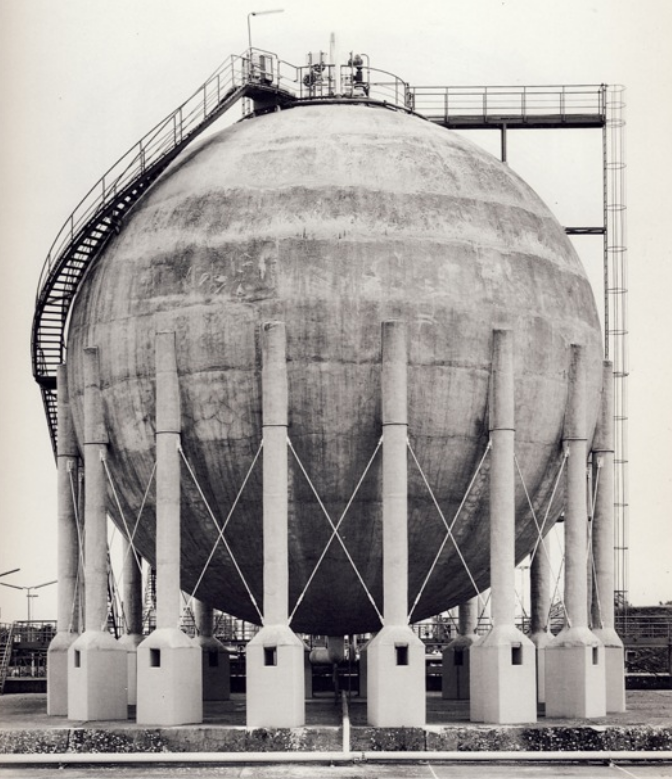
\includegraphics[width=.6\textwidth]{tank.png}
\end{center}

\mynewpage





\begin{question} %% BY L
  Your client wants to know how the \emph{diameter} of the of water tank will
  change if the radius is reduced by $10\%$.
  
    \begin{itemize} 
    \item[\emph{Think:}] Take one minute and answer the following questions. Write down your answers here. When you turn in the assignment, remember to include your original answers from this part.
  \begin{enumerate}
  \item What additional information (if any) do you need/would like
    to answer this question?
    \vspace{1in}
  \item Without looking anything up, what's
    your best guess as to what the answer is?
        \vspace{.5in}

  \item How does your answer above change if we instead increase the
    radius by $10\%$?
        \vspace{.5in}

  \end{enumerate}
  
  \item[\emph{Group:}] Discuss your answers with your group. Do your answers change? What is your group's justification for your answers. Record your responses here.
  
  \vfill
  \item[\emph{Share:}] Have someone from your group share your answers and justifications with the class. Record any changes you would make based on the class discussion.
  \vfill
    \end{itemize}
\end{question}

\mynewpage


\begin{question} %% BY SA
  Your client wants to know how the \emph{cost of the raw materials} for the
  water tank will change if the radius is reduced by $10\%$.
    \begin{itemize} 
    \item[\emph{Think:}] Take one minute and answer the following questions. Write down your answers here. When you turn in the assignment, remember to include your original answers from this part.
  \begin{enumerate}
  \item What additional information (if any) do you need/would like
    to answer this question?
    \vspace{1in}
  \item Without looking anything up, what's
    your best guess as to what the answer is?
        \vspace{.5in}

  \item How does your answer above change if we instead increase the
    radius by $10\%$?
        \vspace{.5in}

  \end{enumerate}
  
  \item[\emph{Group:}] Discuss your answers with your group. Do your answers change? What is your group's justification for your answers. Record your responses here.
  
  \vfill
  \item[\emph{Share:}] Have someone from your group share your answers and justifications with the class. Record any changes you would make based on the class discussion.
  \vfill
    \end{itemize}
\end{question}

\mynewpage


\begin{question} %% BY VOL
  Your client wants to know how the \emph{weight} of the full tank will
  change if the radius is reduced by $10\%$.
    \begin{itemize} 
    \item[\emph{Think:}] Take one minute and answer the following questions. Write down your answers here. When you turn in the assignment, remember to include your original answers from this part.
  \begin{enumerate}
  \item What additional information (if any) do you need/would like
    to answer this question?
    \vspace{1in}
  \item Without looking anything up, what's
    your best guess as to what the answer is?
        \vspace{.5in}

  \item How does your answer above change if we instead increase the
    radius by $10\%$?
        \vspace{.5in}

  \end{enumerate}
  
  \item[\emph{Group:}] Discuss your answers with your group. Do your answers change? What is your group's justification for your answers. Record your responses here.
  
  \vfill
  \item[\emph{Share:}] Have someone from your group share your answers and justifications with the class. Record any changes you would make based on the class discussion.
  \vfill
    \end{itemize}
\end{question}
\end{document}
